\documentclass[tikz,border=2pt]{standalone}
\usepackage{amsmath}
\begin{document}
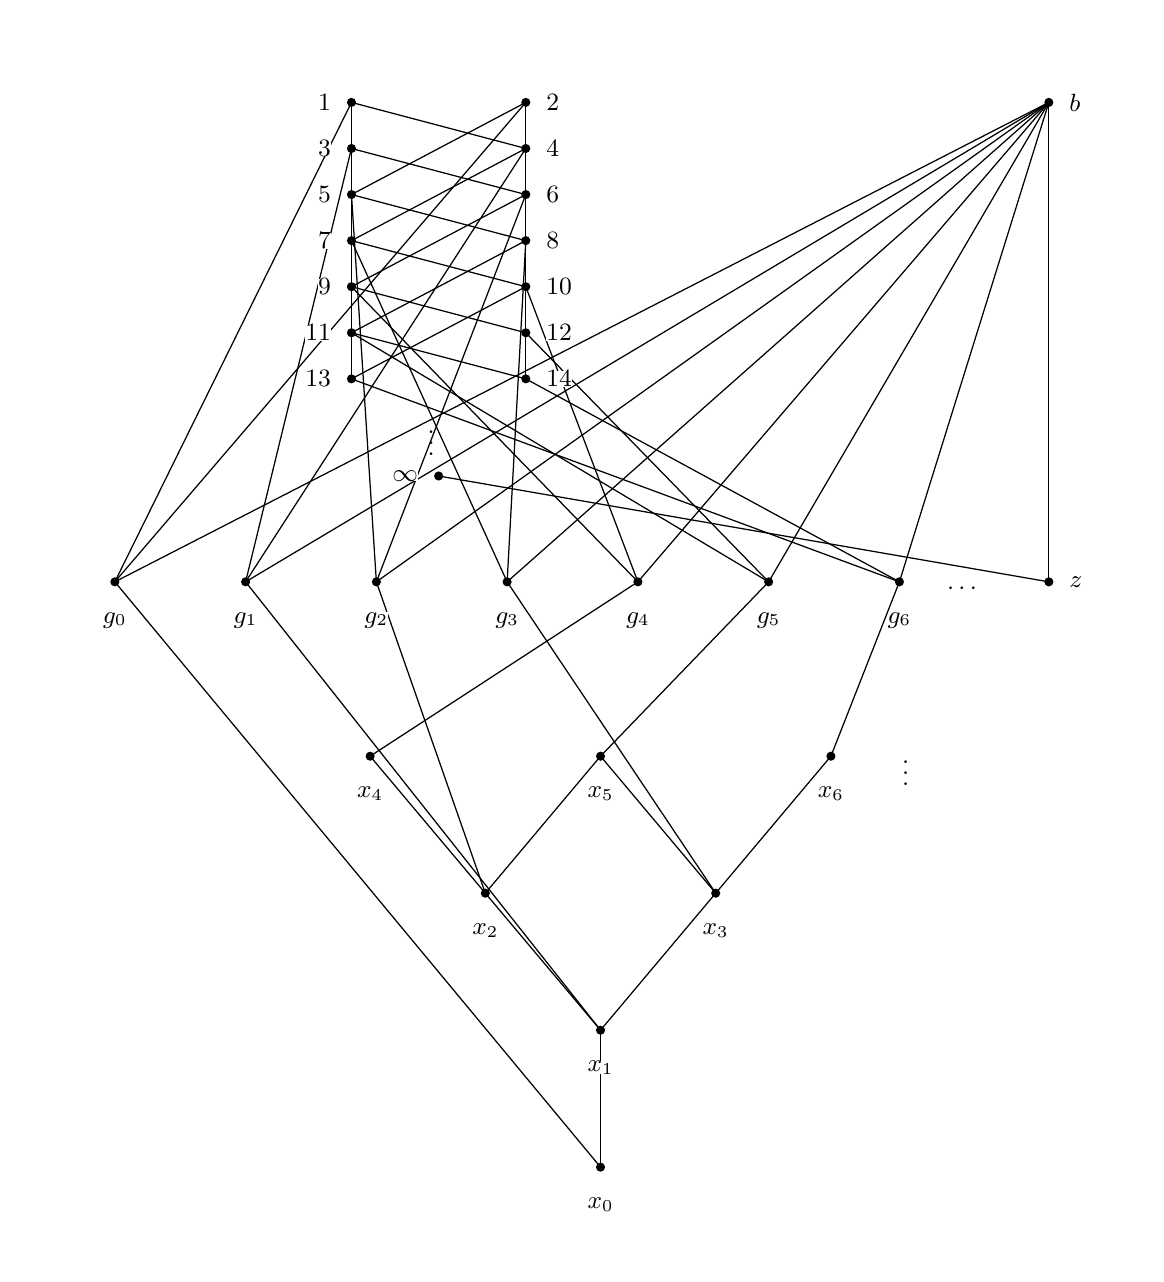
\begin{tikzpicture}[x=.45pt,y=-.45pt,line width=.45pt,line cap=round,font=\fontsize{9}{10}\selectfont]
\path[use as bounding box] (30,15) rectangle (920,1000);
\coordinate (nl1) at (290,75);
\coordinate (nl2) at (430,75);
\coordinate (nl3) at (290,112);
\coordinate (nl4) at (430,112);
\coordinate (nl5) at (290,149);
\coordinate (nl6) at (430,149);
\coordinate (nl7) at (290,186);
\coordinate (nl8) at (430,186);
\coordinate (ninfinity) at (360,375);
\coordinate (nb) at (850,75);
\coordinate (ng0) at (100,460);
\coordinate (ng1) at (205,460);
\coordinate (ng2) at (310,460);
\coordinate (ng3) at (415,460);
\coordinate (ng4) at (520,460);
\coordinate (ng5) at (625,460);
\coordinate (ng6) at (730,460);
\coordinate (ny0) at (490,930);
\coordinate (ny1) at (490,820);
\coordinate (ny2) at (397.5,710);
\coordinate (ny3) at (582.5,710);
\coordinate (ny4) at (305,600);
\coordinate (ny5) at (490,600);
\coordinate (ny6) at (675,600);
\coordinate (nz) at (850,460);
\coordinate (nl9) at (290,223);
\coordinate (nl10) at (430,223);
\coordinate (nl11) at (290,260);
\coordinate (nl12) at (430,260);
\coordinate (nl13) at (290,297);
\coordinate (nl14) at (430,297);
\draw (ng0) -- (nb);
\draw (ng1) -- (nb);
\draw (ng2) -- (nb);
\draw (ng3) -- (nb);
\draw (ng4) -- (nb);
\draw (ng5) -- (nb);
\draw (ng6) -- (nb);
\draw (ny0) -- (ny1);
\draw (ny0) -- (ng0);
\draw (ny1) -- (ny2);
\draw (ny1) -- (ny3);
\draw (ny1) -- (ng1);
\draw (ny2) -- (ny4);
\draw (ny2) -- (ny5);
\draw (ny2) -- (ng2);
\draw (ny3) -- (ny5);
\draw (ny3) -- (ny6);
\draw (ny3) -- (ng3);
\draw (ny4) -- (ng4);
\draw (ny5) -- (ng5);
\draw (ny6) -- (ng6);
\draw (nz) -- (ninfinity);
\draw (nz) -- (nb);
\draw (nl3) -- (nl1);
\draw (nl4) -- (nl1);
\draw (nl4) -- (nl2);
\draw (nl5) -- (nl2);
\draw (nl5) -- (nl3);
\draw (nl6) -- (nl3);
\draw (nl6) -- (nl4);
\draw (nl7) -- (nl4);
\draw (nl7) -- (nl5);
\draw (nl8) -- (nl5);
\draw (nl8) -- (nl6);
\draw (nl9) -- (nl6);
\draw (nl9) -- (nl7);
\draw (nl10) -- (nl7);
\draw (nl10) -- (nl8);
\draw (nl11) -- (nl8);
\draw (nl11) -- (nl9);
\draw (nl12) -- (nl9);
\draw (nl12) -- (nl10);
\draw (nl13) -- (nl10);
\draw (nl13) -- (nl11);
\draw (nl14) -- (nl11);
\draw (nl14) -- (nl12);
\draw (ng0) -- (nl1);
\draw (ng0) -- (nl2);
\draw (ng1) -- (nl3);
\draw (ng1) -- (nl4);
\draw (ng2) -- (nl5);
\draw (ng2) -- (nl6);
\draw (ng3) -- (nl7);
\draw (ng3) -- (nl8);
\draw (ng4) -- (nl9);
\draw (ng4) -- (nl10);
\draw (ng5) -- (nl11);
\draw (ng5) -- (nl12);
\draw (ng6) -- (nl13);
\draw (ng6) -- (nl14);
\node at (354,342) {$\vdots$};
\node at (782,466) {$\cdots$};
\node at (735,607) {$\vdots$};
\fill (nl1) circle[radius=1.65pt];
\node[anchor=east,inner sep=0pt,fill=white] at (274,75) {$1$};
\fill (nl2) circle[radius=1.65pt];
\node[anchor=west,inner sep=0pt,fill=white] at (446,75) {$2$};
\fill (nl3) circle[radius=1.65pt];
\node[anchor=east,inner sep=0pt,fill=white] at (274,112) {$3$};
\fill (nl4) circle[radius=1.65pt];
\node[anchor=west,inner sep=0pt,fill=white] at (446,112) {$4$};
\fill (nl5) circle[radius=1.65pt];
\node[anchor=east,inner sep=0pt,fill=white] at (274,149) {$5$};
\fill (nl6) circle[radius=1.65pt];
\node[anchor=west,inner sep=0pt,fill=white] at (446,149) {$6$};
\fill (nl7) circle[radius=1.65pt];
\node[anchor=east,inner sep=0pt,fill=white] at (274,186) {$7$};
\fill (nl8) circle[radius=1.65pt];
\node[anchor=west,inner sep=0pt,fill=white] at (446,186) {$8$};
\fill (ninfinity) circle[radius=1.65pt];
\node[anchor=east,inner sep=0pt,fill=white] at (344,375) {$\infty$};
\fill (nb) circle[radius=1.65pt];
\node[anchor=west,inner sep=0pt,fill=white] at (866,75) {$b$};
\fill (ng0) circle[radius=1.65pt];
\node[anchor=north,inner sep=0pt,fill=white] at (100,484) {$g_{0}$};
\fill (ng1) circle[radius=1.65pt];
\node[anchor=north,inner sep=0pt,fill=white] at (205,484) {$g_{1}$};
\fill (ng2) circle[radius=1.65pt];
\node[anchor=north,inner sep=0pt,fill=white] at (310,484) {$g_{2}$};
\fill (ng3) circle[radius=1.65pt];
\node[anchor=north,inner sep=0pt,fill=white] at (415,484) {$g_{3}$};
\fill (ng4) circle[radius=1.65pt];
\node[anchor=north,inner sep=0pt,fill=white] at (520,484) {$g_{4}$};
\fill (ng5) circle[radius=1.65pt];
\node[anchor=north,inner sep=0pt,fill=white] at (625,484) {$g_{5}$};
\fill (ng6) circle[radius=1.65pt];
\node[anchor=north,inner sep=0pt,fill=white] at (730,484) {$g_{6}$};
\fill (ny0) circle[radius=1.65pt];
\node[anchor=north,inner sep=0pt,fill=white] at (490,954) {$x_{0}$};
\fill (ny1) circle[radius=1.65pt];
\node[anchor=north,inner sep=0pt,fill=white] at (490,844) {$x_{1}$};
\fill (ny2) circle[radius=1.65pt];
\node[anchor=north,inner sep=0pt,fill=white] at (397.5,734) {$x_{2}$};
\fill (ny3) circle[radius=1.65pt];
\node[anchor=north,inner sep=0pt,fill=white] at (582.5,734) {$x_{3}$};
\fill (ny4) circle[radius=1.65pt];
\node[anchor=north,inner sep=0pt,fill=white] at (305,624) {$x_{4}$};
\fill (ny5) circle[radius=1.65pt];
\node[anchor=north,inner sep=0pt,fill=white] at (490,624) {$x_{5}$};
\fill (ny6) circle[radius=1.65pt];
\node[anchor=north,inner sep=0pt,fill=white] at (675,624) {$x_{6}$};
\fill (nz) circle[radius=1.65pt];
\node[anchor=west,inner sep=0pt,fill=white] at (866,460) {$z$};
\fill (nl9) circle[radius=1.65pt];
\node[anchor=east,inner sep=0pt,fill=white] at (274,223) {$9$};
\fill (nl10) circle[radius=1.65pt];
\node[anchor=west,inner sep=0pt,fill=white] at (446,223) {$10$};
\fill (nl11) circle[radius=1.65pt];
\node[anchor=east,inner sep=0pt,fill=white] at (274,260) {$11$};
\fill (nl12) circle[radius=1.65pt];
\node[anchor=west,inner sep=0pt,fill=white] at (446,260) {$12$};
\fill (nl13) circle[radius=1.65pt];
\node[anchor=east,inner sep=0pt,fill=white] at (274,297) {$13$};
\fill (nl14) circle[radius=1.65pt];
\node[anchor=west,inner sep=0pt,fill=white] at (446,297) {$14$};
\end{tikzpicture}
\end{document}
